\section{Описание интерфейса пользователя}
\setcounter{figure}{0}

Программа разделена на два интерфейса: 
пользовательский, для получения и обработки запросов, 
и администраторский, для редактирования и просмотра баз данных.

Пользовательский интерфейс выполнен в виде интерфейса командной строки. 
Для передачи запроса достаточно сформировать файл по формату, 
описанному выше 
(рис. \ref{request_table}), 
и запустить программу, 
передав параметром путь до сформированного файла. 
Если находяться свободные водитель(и) и грузовик,
подходящие по параметрам в запросе, пользователю будут предоставлены 
их идентифекаторы. Пример успешного запроса на рис. \ref{request_accepted}.

\begin{figure}[hpt!]
    \centering
    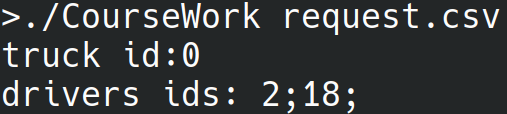
\includegraphics[width=0.7\linewidth]{photo/interface/request_accepted}
    \caption{Пример успешного запроса}
    \label{request_accepted}
\end{figure}

Если в результате обработки запроса не хватит водителей или
не найдётся подходящего грузовика, программа выдаст соответствующее 
сообщение (рис. \ref{request_denied}) и запрос будет отклонён.

\begin{figure}[hpt!]
    \centering
    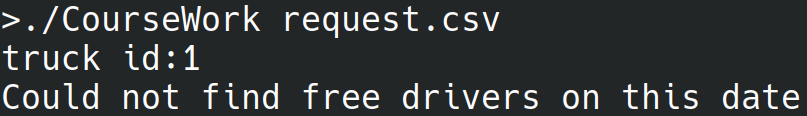
\includegraphics[width=0.7\linewidth]{photo/interface/request_denied}
    \caption{Пример отклонённого запроса}
    \label{request_denied}
\end{figure}

В случае, если дата отправки в запросе уже прошла 
(мы не можем отправить груз вчера),
выводиться соответствующее 
сообщение (рис. \ref{request_late}) и запрос будет отклонён.

\begin{figure}[hpt!]
    \centering
    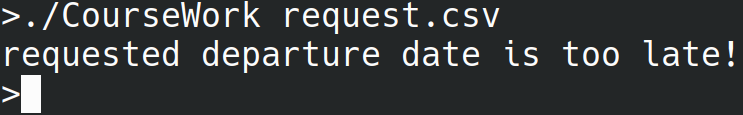
\includegraphics[width=0.7\linewidth]{photo/interface/request_late}
    \caption{Пример позднего запроса}
    \label{request_late}
\end{figure}

Интерфейс администратора выполнен в виде консольного приложения, 
включающего в себя несколько меню для работы с 
базами данных 
(редактирования, добавления, удаления элементов) 
и защиту паролем. 
Администратор обладает правами по манипуляции данными, 
недоступными обычному пользователю. 
Для запуска консоли администратора достаточно 
запустить программу без аргументов. 
После запуска программы предлагается ввести пароль.
В случае успешного ввода пароля пользователь
попадает в лавное меню
(рис. \ref{password_good}).
Иначе пользователю отказывается в доступе
(рис. \ref{password_bad})
Для ввода пароля реалицована функция маски,
то есть вводимые символы заменяются на $ * $.

\begin{figure}[hpt!]
    \centering
    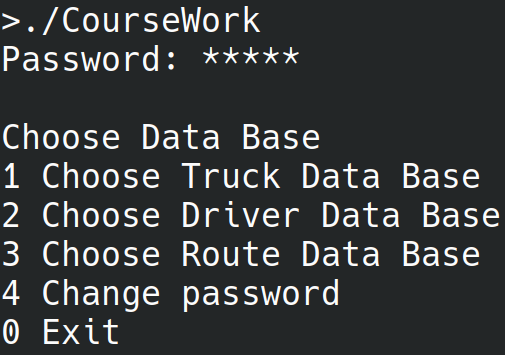
\includegraphics[width=0.7\linewidth]{photo/interface/password_good}
    \caption{Успешный вход в консоль администратора}
    \label{password_good}
\end{figure}

\begin{figure}[hpt!]
    \centering
    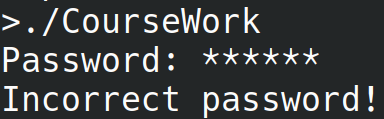
\includegraphics[width=0.7\linewidth]{photo/interface/password_bad}
    \caption{Неудачный вход в консоль администратора}
    \label{password_bad}
\end{figure}

Главное меню (рис. \ref{menu_main}) пердоставляет администротору 
выбор из нескольких баз данных (п. 1-3) и
опцию по смене пароля (п. 4 (рис. \ref{password_change})).

\begin{figure}[H]
    \centering
    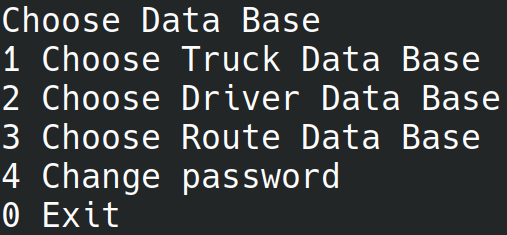
\includegraphics[width=0.7\linewidth]{photo/interface/menu_main}
    \caption{Главное меню}
    \label{menu_main}
\end{figure}

\begin{figure}[H]
    \centering
    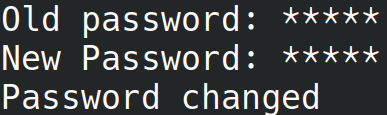
\includegraphics[width=0.7\linewidth]{photo/interface/password_change}
    \caption{Смена пароля}
    \label{password_change}
\end{figure}

Меню для работы с базой данных (рис. \ref{menu_db}) одинаково 
для всех доступных администротору баз данных.

\begin{figure}[H]
    \centering
    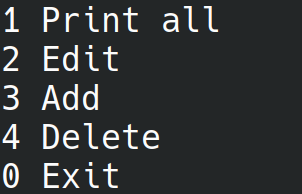
\includegraphics[width=0.7\linewidth]{photo/interface/menu_db}
    \caption{Меню для работы с базой данных}
    \label{menu_db}
\end{figure}

Назначения пунктов меню следующие:

\begin{itemize}
    \item 1 Print all -- вывод базы данных на экран
    \item 2 Edit -- редактирование элемента базы данных
    \item 3 Add -- добавление элемента в базу данных
    \item 4 Delete -- удаление элемента из базы данных
    \item 0 Exit -- возврат в главное меню
\end{itemize}